
% Set document class and necessary packages
\documentclass{article}

% Preamble setup
\usepackage{geometry}
\usepackage{graphicx}
\usepackage{amsmath} % For advanced mathematical formatting (e.g., align*)
\usepackage{amssymb} % For mathematical symbols
\usepackage{amsfonts} % For mathematical fonts
\usepackage{enumitem} % For customizing lists (itemsep)
\usepackage{pdfpages} % For including external PDFs

% Set geometry for 1-inch margins and 6.5 inch text width
\geometry{
    margin=1in,
    textwidth=6.5in
}

% Define title and generate title block
\title{Study Plan for Chemistry Exam 2 (Chapters 5, 8, and 9)}
% No \author or \date required by the prompt
\begin{document}
\maketitle

% Start of Quiz Details section
\subsection*{Quiz Details}
\setlist[itemize]{itemsep=5pt} % Rule 1: Add vertical space between top-level list items
\begin{itemize}
    \item \textbf{Chapter/Topic:} Chapters 5 (Ionic and Covalent Compounds), 8 (Chemical Reactions), and 9 (Chemical reactions in aqueous solutions)
    \item \textbf{Quiz Date and Time:} [Enter Date and Time]
    \item \textbf{Quiz Format:} [e.g., Closed notes, online, in-person]
    \item \textbf{Allowed Materials:} A clean, unmarked copy of \texttt{Periodic Table for testing.pdf}
\end{itemize}
% End of Quiz Details section

\subsection*{Key Topics on the Exam}
\setlist[itemize]{itemsep=5pt} % Rule 1
\begin{itemize}
    \item \textbf{Nomenclature:} Ionic (including Roman numerals and polyatomic ions), Molecular, Binary Acids, Oxoacids, and Hydrates.
    \item \textbf{Formulas \& Moles:} Calculating molar mass, performing conversions ($\text{g} \leftrightarrow \text{mol} \leftrightarrow \text{molecules} \leftrightarrow \text{atoms}$), determining percent mass.
    \item \textbf{Empirical/Molecular Formulas:} Determining empirical formulas from mass data (including combustion analysis results) and deriving molecular formulas from empirical formulas and molecular molar mass.
    \item \textbf{Reactions \& Stoichiometry:} Balancing equations, identifying reaction types, performing mole-to-mole conversions.
    \item \textbf{Limiting Reactants:} Identifying the limiting reagent (LR) and excess reagent (ER), calculating theoretical yield (TY), and calculating excess reagent remaining.
    \item \textbf{Solution Chemistry:} Applied molarity calculations, dilutions ($\text{M}_1\text{V}_1 = \text{M}_2\text{V}_2$), solution stoichiometry (titrations), and $\text{pH}$ and hydronium ion $[\text{H}_3\text{O}^+]$ calculations and classification.
\end{itemize}

\bigskip % Rule 2: Large vertical separation

% Start of Phased Study Plan
\subsection*{Phased Study Plan}

\subsubsection*{Phase 1: Foundation (Nomenclature and Formulaic Rules)}
\setlist[itemize]{itemsep=5pt} % Rule 1
\begin{itemize}
    \item \textbf{Memorization is Critical:} Memorize the polyatomic ions list (from slide 36 in the lecture notes, excluding crossed-off ions). Nomenclature is approximately 20\% of the exam.
    \item Review the predicted charges of main-group elements (excluding transition metals) using the periodic table provided on slide 9 of \texttt{Chapter 5 Lecture Notes.pdf}.
    \item Practice providing names when given formulas, and vice-versa, for all nomenclature types (ionic, molecular, hydrates, acids). Use practice documents like \texttt{Covalent, hydrate, and acid nomenclature Answer Key.pdf} and \texttt{Ionic nomenclature practice Answer Key.pdf}.
    \item Ensure comfort using the criss-cross method to predict ionic formulas based on charges.
\end{itemize}

\bigskip % Rule 2: Large vertical separation

\subsubsection*{Phase 2: Practice \& Application (Stoichiometry Fundamentals)}
\setlist[itemize]{itemsep=5pt} % Rule 1
\begin{itemize}
    \item Master calculations involving molar mass (formula molar mass, $\text{M}$) by summing the contributions of all elements in the chemical formula.
    \item Practice unit conversions: grams $\leftrightarrow$ moles $\leftrightarrow$ molecules $\leftrightarrow$ atoms. See steps illustrated in calculations in \texttt{Excerpts from "Chapter 5 Lecture Notes.pdf"}.
    \item Practice balancing chemical equations. Note that polyatomic ions can sometimes be treated as a single unit during balancing. Use practice problems from \texttt{Types of chemical reactions Answer Key.pdf}.
    \item Review and memorize the classifications of reactions (synthesis, decomposition, single/double replacement, hydrocarbon combustion).
    \item Solve applied molarity problems, calculating molarity ($\text{M} = \text{moles of solute} / \text{liters of solution}$).
\end{itemize}

\bigskip % Rule 2: Large vertical separation

\subsubsection*{Phase 3: Final Mastery (Advanced Calculations and Aqueous Solutions)}
\setlist[itemize]{itemsep=5pt} % Rule 1
\begin{itemize}
    \item \textbf{Limiting Reactants:} Practice identifying the LR and ER by converting reactants to moles of product, and using the reactant that yields the least amount of product to calculate the theoretical yield. Practice calculating the excess reagent remaining. Use examples from \texttt{Reaction stoichiometry worksheet Answer Key.pdf}.
    \item \textbf{Combustion Analysis:} Practice determining the empirical and molecular formulas from the mass percentage data or from masses of $\text{CO}_2$ and $\text{H}_2\text{O}$ produced, especially focusing on handling uneven mole ratios (e.g., multiplying ratios by 2, 3, or 4 when encountering decimals like $.5$, $.33$, or $.25$, respectively).
    \item \textbf{Solution Stoichiometry:} Practice titration calculations, converting between volume and moles using molarity, and applying mole ratios from balanced equations to solve for unknowns. Do not use the dilution formula for titration problems as mole ratios must be considered.
    \item \textbf{Aqueous Solutions:} Practice $\text{M}_1\text{V}_1 = \text{M}_2\text{V}_2$ dilution problems and determining how to properly prepare the final diluted solution.
    \item \textbf{pH:} Calculate $\text{pH}$ given $[\text{H}_3\text{O}^+]$ ($\text{pH} = -\text{log}[\text{H}_3\text{O}^+]$) or calculate $[\text{H}_3\text{O}^+]$ given $\text{pH}$ ($[\text{H}_3\text{O}^+] = 10^{-\text{pH}}$). Remember the ranges for acidic ($\text{pH} < 7.00$) and basic ($\text{pH} > 7.00$) solutions.
\end{itemize}

\bigskip % Rule 2: Large vertical separation
\subsubsection*{Final Preparation Steps}
\setlist[itemize]{itemsep=5pt} % Rule 1
\begin{itemize}
    \item Print a clean, unmarked copy of \texttt{Periodic Table for testing.pdf}.
    \item Review key concepts: Lattice energy depends inversely on atomic radius and directly on ionic charge.
    \item Review homework problems recommended by the instructor for Chapters 5, 8, and 9.
\end{itemize}

\bigskip % Rule 2: Large vertical separation

% Start of Detailed Problem Explanations
\subsection*{Explanations of Practice Problems}

\subsubsection*{Topic: Nomenclature (Ionic with Roman Numerals, Oxoacids, Hydrates)}
\setlist[itemize]{itemsep=5pt} % Rule 1

\begin{itemize}
    \item \textbf{Problem: Name $\text{AuBr}_3$}
    \item \textbf{Explanation:} This is an ionic compound. Since Gold ($\text{Au}$) is a transition metal, the Stock system using Roman numerals is required to indicate the charge on the cation. Bromine ($\text{Br}$) forms the anion bromide ($\text{Br}^-$). Since there are three bromide ions (total charge $-3$), the gold cation must have a $+3$ charge ($\text{Au}^{3+}$) to maintain electrical neutrality. The name is \textbf{Gold (III) bromide}.

    \item \textbf{Problem: Name $\text{HNO}_2$}
    \item \textbf{Explanation:} This is an oxoacid. Identify the polyatomic anion: $\text{NO}_2^-$ is the nitrite ion. An acid formed from an oxoanion ending in ``ite'' ends in ``ous acid''. Thus, the name is \textbf{Nitrous acid}.

    \item \textbf{Problem: Write the formula for Iron (III) phosphate tetrahydrate}
    \item \textbf{Explanation:} This compound is a hydrate, which is an ionic compound containing a specific number of water molecules in its chemical formula. The ionic part is Iron (III) phosphate. Iron (III) is $\text{Fe}^{3+}$. Phosphate is $\text{PO}_4^{3-}$. Since the charges cancel, the ionic formula is $\text{FePO}_4$. The prefix "tetra" denotes four water molecules, $\cdot 4\text{H}_2\text{O}$. The formula is \textbf{$\text{FePO}_4 \cdot 4\text{H}_2\text{O}$}.
\end{itemize}

\bigskip % Rule 2: Large vertical separation

\subsubsection*{Topic: Empirical and Molecular Formula Determination}
\setlist[itemize]{itemsep=5pt} % Rule 1

\begin{itemize}
    \item \textbf{Problem: A compound is 72.2\% magnesium and 27.8\% nitrogen by mass. Determine the empirical formula.} (Source: \texttt{Empirical and molecular formulae Answer Key.pdf}, Problem 1)

    \item \textbf{Explanation:} Assume a 100 $\text{g}$ sample (72.2 $\text{g}$ $\text{Mg}$ and 27.8 $\text{g}$ $\text{N}$) and convert masses to moles using molar masses ($\text{Mg} = 24.305 \text{ g/mol}$; $\text{N} = 14.007 \text{ g/mol}$).
    \begin{align*}
        \text{Moles Mg} &= 72.2 \text{ g Mg} \times \frac{1 \text{ mole Mg}}{24.305 \text{ g Mg}} \approx 2.971 \text{ moles Mg} \\
        \text{Moles N} &= 27.8 \text{ g N} \times \frac{1 \text{ mole N}}{14.007 \text{ g N}} \approx 1.985 \text{ moles N}
    \end{align*}
    Divide by the smallest number of moles ($\text{N} = 1.985$ moles):
    \begin{align*}
        \text{Mg}: \frac{2.971}{1.985} &\approx 1.50 \\
        \text{N}: \frac{1.985}{1.985} &= 1.00
    \end{align*}
    Since the mole ratio contains $1.5$, multiply both ratios by $2$ to obtain whole numbers (a rule of thumb for $.5$ decimals is to multiply by $2$).
    \begin{align*}
        \text{Mg}: 1.50 \times 2 &= 3 \\
        \text{N}: 1.00 \times 2 &= 2
    \end{align*}
    The empirical formula is \textbf{$\text{Mg}_3\text{N}_2$}.

    \item \textbf{Problem: A compound has an empirical formula of $\text{NO}_2$ and a molar mass of $92.02 \text{ g/mol}$. Determine the molecular formula.} (Source: \texttt{Empirical and molecular formulae Answer Key.pdf}, Problem 5)

    \item \textbf{Explanation:} The relationship between the molecular formula molar mass and the empirical formula molar mass determines the multiplier needed.
    \begin{enumerate}
        \item Calculate the empirical formula molar mass ($\text{NO}_2$):
        \begin{align*}
            \text{Molar Mass } (\text{NO}_2) &= 1(\text{Atomic mass of N}) + 2(\text{Atomic mass of O}) \\
            &= 1(14.007 \text{ g/mol}) + 2(15.999 \text{ g/mol}) \\
            &\approx 46.005 \text{ g/mol}
        \end{align*}
        \item Calculate the ratio of the molecular molar mass to the empirical molar mass:
        \begin{align*}
            \text{Ratio} &= \frac{92.02 \text{ g/mol}}{46.005 \text{ g/mol}} \approx 2.000
        \end{align*}
        \item Multiply the subscripts in the empirical formula ($\text{NO}_2$) by the ratio (2): $2 \times \text{NO}_2 = \text{N}_2\text{O}_4$.
    \end{enumerate}
    The molecular formula is \textbf{$\text{N}_2\text{O}_4$}.

\end{itemize}

\bigskip % Rule 2: Large vertical separation

\subsubsection*{Topic: Limiting Reagents and Percent Yield}
\setlist[itemize]{itemsep=5pt} % Rule 1

\begin{itemize}
    \item \textbf{Problem: When $15.0 \text{ g}$ of $\text{CuCl}_2$ reacts with $20.0 \text{ g}$ of $\text{NaNO}_3$, how much $\text{Cu}(\text{NO}_3)_2$ can be formed? If $11.3 \text{ g}$ of $\text{Cu}(\text{NO}_3)_2$ are formed, what is the percent yield?} (Source: \texttt{Reaction stoichiometry worksheet Answer Key.pdf}, Problem 1)

    \item \textbf{Balanced Equation:} $\text{CuCl}_2 + 2\text{NaNO}_3 \rightarrow \text{Cu}(\text{NO}_3)_2 + 2\text{NaCl}$

    \item \textbf{Explanation: Determining the Limiting Reagent and Theoretical Yield}
    \begin{enumerate}
        \item Calculate moles of product ($\text{Cu}(\text{NO}_3)_2$) formed from each reactant (Molar masses: $\text{CuCl}_2 = 134.45 \text{ g/mol}$, $\text{NaNO}_3 = 84.99 \text{ g/mol}$).
        \begin{align*}
            \text{Moles Cu}(\text{NO}_3)_2 \text{ from CuCl}_2 &= 15.0 \text{ g } \text{CuCl}_2 \times \frac{1 \text{ mol } \text{CuCl}_2}{134.45 \text{ g}} \times \frac{1 \text{ mol } \text{Cu}(\text{NO}_3)_2}{1 \text{ mol } \text{CuCl}_2} \approx 0.1116 \text{ mol} \\
            \text{Moles Cu}(\text{NO}_3)_2 \text{ from NaNO}_3 &= 20.0 \text{ g } \text{NaNO}_3 \times \frac{1 \text{ mol } \text{NaNO}_3}{84.99 \text{ g}} \times \frac{1 \text{ mol } \text{Cu}(\text{NO}_3)_2}{2 \text{ mol } \text{NaNO}_3} \approx 0.1177 \text{ mol}
        \end{align*}
        \item Since $0.1116 \text{ mol}$ is the smallest amount of product, $\text{CuCl}_2$ is the \textbf{limiting reagent}.
        \item Calculate the theoretical yield (TY) in grams (Molar mass $\text{Cu}(\text{NO}_3)_2 = 187.56 \text{ g/mol}$).
        \begin{align*}
            \text{TY } \text{Cu}(\text{NO}_3)_2 &= 0.1116 \text{ mol} \times \frac{187.56 \text{ g}}{1 \text{ mol}} \approx \textbf{20.9 g } \text{Cu}(\text{NO}_3)_2
        \end{align*}
    \item \textbf{Explanation: Calculating Excess Reagent Remaining}
    \begin{enumerate}
        \item Calculate the mass of the excess reagent ($\text{NaNO}_3$) consumed by the limiting reagent ($\text{CuCl}_2$):
        \begin{align*}
            \text{Mass NaNO}_3 \text{ used} &= 15.0 \text{ g } \text{CuCl}_2 \times \frac{1 \text{ mol } \text{CuCl}_2}{134.45 \text{ g}} \times \frac{2 \text{ mol } \text{NaNO}_3}{1 \text{ mol } \text{CuCl}_2} \times \frac{84.99 \text{ g}}{1 \text{ mol } \text{NaNO}_3} \approx 19.0 \text{ g}
        \end{align*}
        \item Subtract mass used from initial mass:
        \begin{align*}
            \text{Mass remaining} &= 20.0 \text{ g } (\text{initial}) - 19.0 \text{ g } (\text{used}) = \textbf{1.0 g } \text{NaNO}_3 \text{ (left over)}
        \end{align*}
    \item \textbf{Explanation: Calculating Percent Yield}
    \begin{enumerate}
        \item Use the formula $\text{Percent Yield} = \frac{\text{Actual Yield}}{\text{Theoretical Yield}} \times 100\%$.
        \begin{align*}
            \text{\% Yield} &= \frac{11.3 \text{ g}}{20.9 \text{ g}} \times 100\% \approx \textbf{54.0\%}
        \end{align*}
    \end{enumerate}
\end{itemize}

\bigskip % Rule 2: Large vertical separation

\subsubsection*{Topic: Solution Stoichiometry and Dilution}
\setlist[itemize]{itemsep=5pt} % Rule 1

\begin{itemize}
    \item \textbf{Problem 1: Calculate the final volume to dilute $30.0 \text{ mL}$ of a $12 \text{ M}$ $\text{HCl}$ solution to make a $0.35 \text{ M}$ solution.} (Source: \texttt{Molarity, dilutions, and solution stoichiometry Answer Key.pdf}, Problem 3)

    \item \textbf{Explanation:} This is a dilution problem, requiring the use of the formula $\text{M}_1\text{V}_1 = \text{M}_2\text{V}_2$.
    \begin{align*}
        \text{V}_2 &= \frac{\text{M}_1\text{V}_1}{\text{M}_2} \\
        \text{V}_2 &= \frac{(12 \text{ M})(30.0 \text{ mL})}{0.35 \text{ M}} \\
        \text{V}_2 &\approx \textbf{1.0} \times \mathbf{10^3 \text{ mL}} \text{ (or } 1000 \text{ mL)}
    \end{align*}

    \item \textbf{Problem 2: What is the volume (in $\text{mL}$) of $1.2 \text{ M}$ $\text{HCl}$ needed to dissolve $5.8 \text{ g}$ $\text{Al}(\text{OH})_3$? The reaction is: $\text{Al}(\text{OH})_3(\text{s}) + 3\text{HCl}(\text{aq}) \rightarrow \text{AlCl}_3(\text{aq}) + 3\text{H}_2\text{O}(\text{l})$} (Source: \texttt{Molarity, dilutions, and solution stoichiometry Answer Key.pdf}, Problem 6)

    \item \textbf{Explanation:} This requires solution stoichiometry ($\text{g} \rightarrow \text{mol } \text{Al}(\text{OH})_3 \rightarrow \text{mol } \text{HCl} \rightarrow \text{L } \text{HCl}$). (Molar masses: $\text{Al}(\text{OH})_3 \approx 78.00 \text{ g/mol}$).
    \begin{align*}
        \text{Volume HCl} &= 5.8 \text{ g } \text{Al}(\text{OH})_3 \times \frac{1 \text{ mol } \text{Al}(\text{OH})_3}{78.00 \text{ g}} \times \frac{3 \text{ mol } \text{HCl}}{1 \text{ mol } \text{Al}(\text{OH})_3} \\
        &\times \frac{1 \text{ L}}{1.2 \text{ moles } \text{HCl}} \times \frac{1000 \text{ mL}}{1 \text{ L}} \\
        &\approx \textbf{190 mL} \text{ (or } 1.9 \times 10^2 \text{ mL)}
    \end{align*}
\end{itemize}

\bigskip % Rule 2: Large vertical separation

\subsubsection*{Topic: pH and Hydronium Concentration}
\setlist[itemize]{itemsep=5pt} % Rule 1

\begin{itemize}
    \item \textbf{Problem 1: Calculate the $\text{pH}$ for $[\text{H}_3\text{O}^+] = 4.3 \times 10^{-8} \text{ M}$ and classify the solution.} (Source: \texttt{Chapter 9 Lecture Notes.pdf}, Practice a)

    \item \textbf{Explanation:} Use the definition $\text{pH} = -\text{log}[\text{H}_3\text{O}^+]$.
    \begin{align*}
        \text{pH} &= -\text{log}[4.3 \times 10^{-8} \text{ M}] \\
        \text{pH} &= \textbf{7.37}
    \end{align*}
    Since $\text{pH} > 7.00$, the solution is \textbf{basic}.

    \item \textbf{Problem 2: Calculate $[\text{H}_3\text{O}^+]$ concentration for $\text{pH} = 9.65$.} (Source: \texttt{Chapter 9 Lecture Notes.pdf}, Practice a)

    \item \textbf{Explanation:} Use the inverse relationship $[\text{H}_3\text{O}^+] = 10^{-\text{pH}}$.
    \begin{align*}
        [\text{H}_3\text{O}^+] &= 10^{-9.65} \\
        [\text{H}_3\text{O}^+] &\approx \textbf{2.2} \times \mathbf{10^{-10} \text{ M}}
    \end{align*}
\end{itemize}

\bigskip % Rule 2: Large vertical separation

% Inclusion of the periodic table PDF as required
\newpage
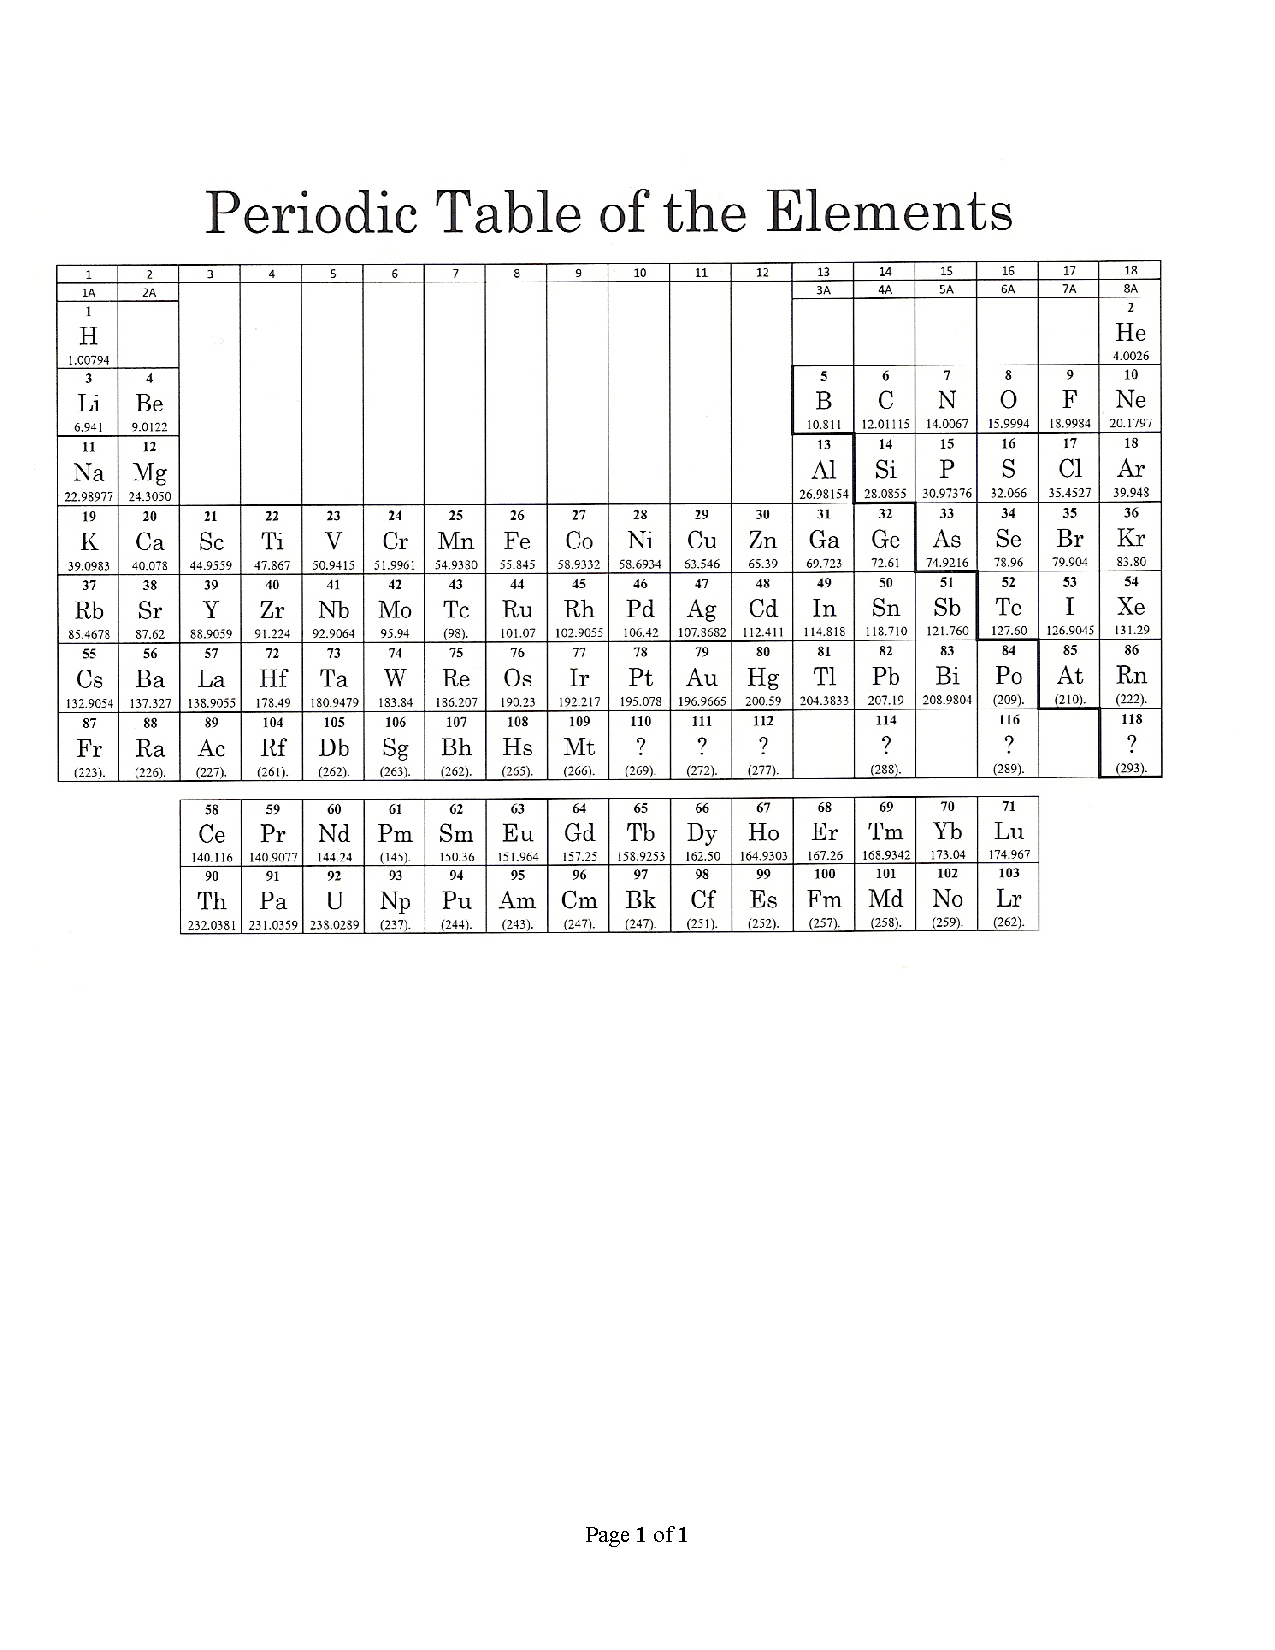
\includepdf[pages={-}]{Periodic Table for testing.pdf}

\end{document}
```